%% GeoFDI manuscript, v0 (Sprint 10). Working title; author block is a placeholder. Single-blind: no anonymisation.
\documentclass[conference]{IEEEtran}
\IEEEoverridecommandlockouts

\usepackage{cite}
\usepackage{amsmath,amssymb,amsfonts,amsthm}
\usepackage{algorithm}
\usepackage{algpseudocode}
\usepackage{graphicx}
\usepackage{booktabs}
\usepackage{multirow}
\usepackage{tikz}
\usetikzlibrary{arrows.meta,positioning,fit,backgrounds,calc,shapes.geometric}
\usepackage[framemethod=TikZ]{mdframed}
\usepackage{xcolor}
\usepackage{url}
\usepackage[hidelinks]{hyperref}
\usepackage{cleveref}

% ---------------------------------------------------------------- macros (kept identical to theory/preamble.tex)
\newcommand{\symgrp}{\Sigma}
\newcommand{\gs}{g_{\mathrm{s}}}
\newcommand{\repW}{\rho_{\mathcal{W}}}
\newcommand{\R}{\mathbb{R}}
\newcommand{\SE}{\mathrm{SE}}
\newcommand{\SO}{\mathrm{SO}}
\newcommand{\eps}[1]{\varepsilon_{\mathrm{#1}}}
\newcommand{\push}[1]{{#1}_{\#}}
\newcommand{\Rminus}{R^{-}}
\newcommand{\Rplus}{R^{+}}
\newcommand{\Law}{\mathcal{L}}
\newcommand{\Tc}{T_{\mathrm{c}}}

\newtheorem{theorem}{Theorem}
\newtheorem{proposition}[theorem]{Proposition}
\newtheorem{corollary}[theorem]{Corollary}
\newtheorem{lemma}[theorem]{Lemma}
\theoremstyle{definition}
\newtheorem{definition}[theorem]{Definition}
\newtheorem{assumption}{Assumption}
\theoremstyle{remark}
\newtheorem{remark}[theorem]{Remark}

% a visible box for data we have not collected yet (Sprint 10: the robot-day list)
\newmdenv[linecolor=black!55,linewidth=0.6pt,backgroundcolor=black!4,innertopmargin=4pt,innerbottommargin=4pt,
          skipabove=6pt,skipbelow=6pt,roundcorner=2pt]{placeholderbox}

\begin{document}

\title{GeoFDI: Fault and Slip Detection as Invariance Testing,\\
with Finite-Sample Guarantees for Legged and\\ Wheeled-Legged Robots}

\author{\IEEEauthorblockN{Kaiwen Yang}
\IEEEauthorblockA{[affiliation TBD]\\ \texttt{[email TBD]}}
\and
\IEEEauthorblockN{[advisor TBD]}
\IEEEauthorblockA{[affiliation TBD]}}

\maketitle

\begin{abstract}
Legged robots degrade silently: an actuator loses torque, a foot slips for part of a step, an encoder drifts. Existing
detectors either threshold a model residual against a distributional assumption a periodic robot violates, or learn what
nominal looks like and threshold that; in both cases the false-alarm rate is empirical, and we measure it missing its
target by $3\times$ to $10\times$. We reframe detection as \emph{testing the structural invariances of the robot
itself}: the mirror symmetry of the body, the space--time symmetry of the commanded gait, and the geometry of contact.
Faults and slip are, by construction, breaks of these, so a group-randomisation test of the invariance hypothesis yields
a false-alarm rate that is \emph{exact at any sample size}, requires no fault data and no training, and extends to an
anytime-valid sequential monitor. Because the group is explicit we can characterise what such a test can see: we prove a
two-layer dichotomy separating faults that are invisible to \emph{every} invariance test from those any consistent
statistic detects, which forces a three-channel architecture and dictates when a learned nominal model must be
equivariant. We further prove that a rolling contact preserves the group-affine structure of a contact-aided invariant
filter, admitting wheeled-legged robots to the same machinery. Evaluation spans a mirror-exact simulator, three public
datasets (Mini Cheetah, Leg-KILO Go1, Cerberus A1) and two of our own platforms. On an external fault dataset the test
holds its level at $0.049$ where a Mahalanobis detector fires on $52\,\%$ of healthy segments; on our own Go2, eleven
sessions across three sites and two months, the recalibrated asymmetry level reproduces to within a factor $1.18$; on
our wheeled-legged M1 the rolling-contact filter recovers $0.99$--$1.00$ of the driven path where the standard
fixed-foot filter recovers $0.03$; and as an estimator front-end the calibrated per-event gate discards $1.9\,\%$ of
nominal contact measurements against $40.6\,\%$ for the standard fixed foot-speed threshold.

\end{abstract}

\section{Introduction}
\label{sec:intro}

A legged robot's usefulness outside a laboratory rests on two things it cannot observe directly: whether its actuators
still deliver what the controller asks, and whether its feet are where the estimator believes they are. Both degrade
silently. An actuator loses torque gradually; a foot slips for a fraction of a step on a wet tile; an encoder drifts by
a few milliradians. None of these announce themselves, and each corrupts the state estimate and the controller that
depends on it.

% Fig. 1 — the whole claim in one single-column figure (Sprint 10 W2.2).
% Left: three structural invariances a healthy robot must satisfy. Middle: breaking one IS the fault/slip.
% Right: the three channels that read the break, and what each delivers.
\begin{figure}[t]
\centering
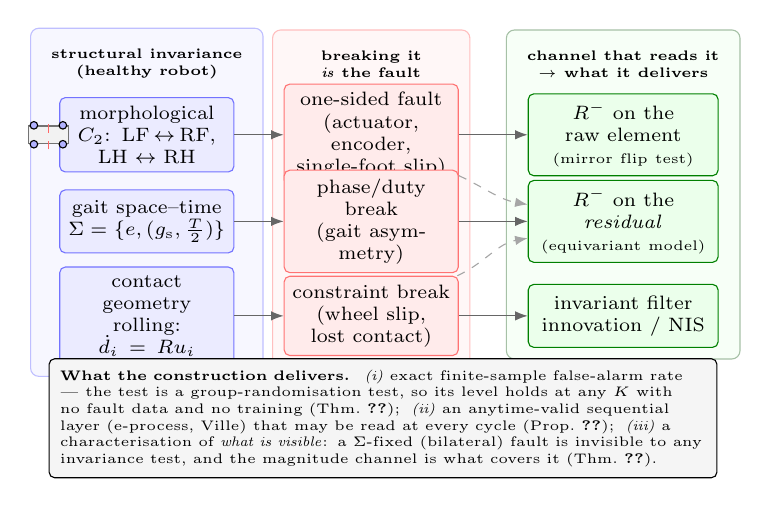
\begin{tikzpicture}[
  font=\scriptsize,
  box/.style={draw,rounded corners=2pt,align=center,inner sep=3pt,minimum height=8mm,text width=20mm},
  inv/.style={box,fill=blue!8,draw=blue!55},
  brk/.style={box,fill=red!8,draw=red!55,text width=20mm},
  ch/.style={box,fill=green!8,draw=green!50!black,text width=22mm},
  del/.style={align=left,inner sep=1pt,font=\tiny},
  ar/.style={-{Latex[length=1.6mm]},draw=black!60},
  lbl/.style={font=\tiny\bfseries,align=center}
]

% ---------------- column headings
\node[lbl] (h1) at (0,2.35) {structural invariance\\(healthy robot)};
\node[lbl] (h2) at (2.85,2.35) {breaking it\\\emph{is} the fault};
\node[lbl] (h3) at (6.05,2.35) {channel that reads it\\$\rightarrow$ what it delivers};

% ---------------- left: three invariances
\node[inv] (i1) at (0,1.45) {morphological\\$C_2$: $\mathrm{LF}\!\leftrightarrow\!\mathrm{RF}$, $\mathrm{LH}\!\leftrightarrow\!\mathrm{RH}$};
\node[inv] (i2) at (0,0.35) {gait space--time\\$\symgrp=\{e,(\gs,\tfrac{T}{2})\}$};
\node[inv] (i3) at (0,-0.85) {contact geometry\\rolling: $\dot d_i = R u_i$};

% tiny quadruped pictogram inside i1's margin
\begin{scope}[shift={(-1.25,1.45)},scale=0.16]
  \draw[black!55,fill=black!5] (-1.6,-0.7) rectangle (1.6,0.7);
  \draw[dashed,red!60] (0,-1.15) -- (0,1.15);
  \foreach \x/\y in {-1.15/0.75,1.15/0.75,-1.15/-0.75,1.15/-0.75} \draw[fill=blue!30] (\x,\y) circle (0.3);
\end{scope}

% ---------------- middle: the break
\node[brk] (b1) at (2.85,1.45) {one-sided fault\\(actuator, encoder,\\single-foot slip)};
\node[brk] (b2) at (2.85,0.35) {phase/duty break\\(gait asymmetry)};
\node[brk] (b3) at (2.85,-0.85) {constraint break\\(wheel slip, lost contact)};

% ---------------- right: channels
\node[ch] (c1) at (6.05,1.45) {$\Rminus$ on the raw element\\{\tiny(mirror flip test)}};
\node[ch] (c2) at (6.05,0.35) {$\Rminus$ on the \emph{residual}\\{\tiny(equivariant model)}};
\node[ch] (c3) at (6.05,-0.85) {invariant filter\\innovation / NIS};

% ---------------- arrows
\foreach \a/\b in {i1/b1,i2/b2,i3/b3} \draw[ar] (\a) -- (\b);
\foreach \a/\b in {b1/c1,b2/c2,b3/c3} \draw[ar] (\a) -- (\b);
% cross links: the residual channel also serves the one-sided fault; the filter also serves the gait break
\draw[ar,dashed,black!35] (b1) to[out=-25,in=170] (c2);
\draw[ar,dashed,black!35] (b3) to[out=25,in=190] (c2);

% ---------------- deliverables strip
\node[draw,fill=black!4,rounded corners=2pt,text width=82mm,align=left,inner sep=4pt,font=\tiny]
  (dl) at (3.0,-2.15) {%
  \textbf{What the construction delivers.}\;
  \emph{(i)} exact finite-sample false-alarm rate --- the test is a group-randomisation test, so its level holds at any
  $K$ with no fault data and no training (Thm.~\ref{thm:exact});\;
  \emph{(ii)} an anytime-valid sequential layer (e-process, Ville) that may be read at every cycle
  (Prop.~\ref{prop:seq});\;
  \emph{(iii)} a characterisation of \emph{what is visible}: a $\symgrp$-fixed (bilateral) fault is invisible to any
  invariance test, and the magnitude channel is what covers it (Thm.~\ref{thm:twolayer}).};

\begin{scope}[on background layer]
  \node[fit=(h1)(i3),draw=blue!25,rounded corners=3pt,inner sep=4pt,fill=blue!3] {};
  \node[fit=(h2)(b3),draw=red!25,rounded corners=3pt,inner sep=4pt,fill=red!3] {};
  \node[fit=(h3)(c3),draw=green!30!black!35,rounded corners=3pt,inner sep=4pt,fill=green!3] {};
\end{scope}
\end{tikzpicture}
\caption{\textbf{Fault and slip detection as invariance testing.} A healthy legged or wheeled-legged robot satisfies
three structural invariances (left): the morphological mirror symmetry of the body, the space--time symmetry of the
commanded gait, and the geometry of contact (a stance foot is fixed; a rolling wheel's contact point moves at the
measured rolling rate). Every fault or slip we target \emph{is} a break of one of them (middle), which turns detection
into a test of a symmetry hypothesis rather than a comparison against a learned or thresholded nominal. Three channels
read the break (right); dashed links mark the couplings that make them complementary rather than redundant.}
\label{fig:concept}
\end{figure}


The established answers fall into two families, and both leave the same hole. \emph{Model-based} residual methods run a
dynamics model --- a generalised-momentum observer is the canonical choice
\cite{deluca2003actuator,haddadin2017robot} --- and threshold the residual, usually against a $\chi^2$ quantile.
\emph{Data-driven} methods learn what nominal looks like, from an autoencoder or a recurrent classifier, and threshold a
reconstruction error or a predicted fault parameter. The hole is the false-alarm rate. A $\chi^2$ threshold is exact
only if the residual is i.i.d.\ Gaussian, and a legged robot's residual is neither: it is gait-periodic, serially
correlated, and non-stationary across a recording. We measure the consequence directly. On our simulation benchmark the
textbook momentum-observer $\chi^2$ detector runs at a nominal alarm rate of \textbf{0.15} against a nominal $0.05$, and
re-calibrating its threshold on the robot's own nominal data does not repair it --- on a \emph{held-out} stretch of the
same nominal recording the rate is \textbf{0.50}, because the residual's statistics have already moved
(\S\ref{sec:simulation}). On an external, third-party fault dataset a Mahalanobis detector fires on \textbf{52\,\%} of
healthy segments (0.522 false alarms per healthy gap) where our test fires on \textbf{4.9\,\%}, i.e.\ at its nominal
level (\S\ref{sec:external}). A detector whose false-alarm rate is unknown cannot be given authority over a controller,
which is why slip handling in practice is still a hand-tuned threshold on foot speed \cite{jenelten2019slippery}.

\paragraph{Gap}
Three literatures each hold one piece and none holds the combination. Morphological-symmetry work in robotics
\cite{ordonez2023discrete} uses a robot's discrete symmetry group to constrain models and policies, but treats symmetry
as an architectural prior, not as a hypothesis to be tested. Fault detection and contact estimation
\cite{camurri2017probabilistic,lin2021contact} build ever better nominal models and contact classifiers, but calibrate
their decisions empirically. Invariance testing in statistics \cite{hemerik2018exact,koning2023evalues} gives exactly
the guarantee the robotics side lacks --- a group-randomisation test whose level is exact in finite samples, and an
anytime-valid sequential form --- but has not been connected to a physical invariance a robot actually possesses. The
missing step is to notice that a healthy legged robot \emph{already satisfies} a group invariance precisely enough to
serve as the null hypothesis, and that the faults we care about are exactly the things that break it.

\paragraph{Thesis}
We propose to detect faults and slip by testing the structural invariances of the robot itself (Fig.~\ref{fig:concept}).
The morphological mirror symmetry of the body, the space--time symmetry of the commanded gait, and the geometry of
contact are properties a healthy machine must satisfy; a one-sided actuator fault, a single-foot slip, or a broken
rolling constraint are, by construction, violations of them. Framing detection this way replaces a learned or
thresholded nominal with a hypothesis that needs no fault data, no training, and --- in its model-free form --- no
dynamics model, and it inherits an exact finite-sample false-alarm rate from the group-randomisation construction.

\paragraph{Contributions}
\begin{enumerate}
\item \textbf{Invariance as the null, with an exact level.} We formulate the healthy-robot hypothesis $H_0$ as
  distributional invariance of a phase-registered data element under the gait symmetry group, and test it with a
  group-randomisation (flip) test whose false-alarm rate is \emph{exact at any sample size}, plus an anytime-valid
  sequential layer built from e-processes. We also give the recalibrated null $H_0'$ for the realistic case of a robot
  that is stably but measurably asymmetric, and a power lower bound with an explicit sample-size rule
  (\S\ref{sec:theory}; Thm.~\ref{thm:exact}, Prop.~\ref{prop:power}, Prop.~\ref{prop:seq}).
\item \textbf{A two-layer characterisation of what is visible, and the architecture it forces.} We prove a dichotomy:
  a fault fixed by the symmetry group (a bilaterally symmetric degradation) is invisible to \emph{every} invariance
  test, whatever its magnitude, provided the faulted loop keeps a unique symmetric attractor; anything that breaks the
  law is detectable by a consistent statistic. The mean-level layer gives the power of the specific paired statistic,
  and the two layers do not coincide --- a zero-mean law change is invisible to the paired statistic and visible to an
  energy-distance one. This is why the system needs three channels rather than one
  (\S\ref{sec:theory}; Thm.~\ref{thm:twolayer}).
\item \textbf{Equivariant nominal models, and why equivariance is not optional.} When a learned dynamics model is used
  to form a residual, we show the residual inherits $H_0$ only if the model is equivariant, quantify the contamination
  a non-equivariant model injects, and construct an equivariant Deep Lagrangian Network by mirror weight sharing. The
  effect is not marginal: a plain learned model drives the residual test's false-alarm rate to $1.00$ while its
  equivariant twin stays at $0.00$ (\S\ref{sec:theory},~\S\ref{sec:simulation}).
\item \textbf{Rolling contact preserves the invariant filter, and a five-layer evidence stack.} We prove that a rolling
  wheel's moving contact keeps the contact-aided invariant filter group-affine --- the invariant error dynamics is
  unchanged, only the mean and the process noise move --- which admits wheeled-legged robots to the same estimator and
  the same gating front-end as point-foot robots. The claims are evaluated at five levels of increasing externality,
  including \emph{two} of our own hardware platforms (\S\ref{sec:hardware}).
\end{enumerate}

\paragraph{What the evaluation shows}
On our own Unitree Go2 corpus --- eleven sessions, a machine over a year in service, three sites, two dates two months
apart --- the naive invariance test rejects on \textbf{11/11} sessions, i.e.\ it sees the machine's real, stable
left--right asymmetry, and the recalibrated level $\nu_0$ reproduces across the two-month gap to within a factor
\textbf{1.18}, which is smaller than the session-to-session spread within a single day. On the wheeled-legged M1 the
rolling-contact filter recovers \textbf{0.99--1.00} of the driven path length where a fixed-foot filter recovers
\textbf{0.03--0.04}. Used as an estimator front-end, the calibrated per-event gate discards \textbf{1.9\,\%} of nominal
contact measurements where the standard fixed foot-speed threshold discards \textbf{40.6\,\%} of them on the same real
outdoor data. And on the external benchmark the test holds its level at \textbf{0.049} against a nominal $0.05$.

\section{Related Work}
\label{sec:related}
[placeholder]

\section{Preliminaries}
\label{sec:preliminaries}
[placeholder]

\section{Theory}
\label{sec:theory}

This section states the results and the intuition; every proof is in Appendix~\ref{app:proofs}, which also carries the
map from the numbering here to the numbering of the technical notes.

\subsection{An exact test, at any sample size}

\begin{theorem}[Exactness of the flip test]
\label{thm:exact}
Let $Z_1,\dots,Z_K$ be data elements that are exchangeable under $H_0$, and let $T$ be any statistic. Draw $M-1$ i.i.d.\
uniform group elements $\sigma_m\in\symgrp$ (equivalently, i.i.d.\ signs on the antisymmetric component) and let
$p=\frac{1}{M}\bigl(1+\#\{m: T(\rho(\sigma_m)Z)\ge T(Z)\}\bigr)$. Then under $H_0$, $\mathbb{P}(p\le\alpha)\le\alpha$
for every $K$ and every $M$, with equality when $\alpha M$ is an integer.
\end{theorem}
The mechanism is that under $H_0$ the observed configuration and its group images are equally likely, so the rank of the
observed statistic among its own orbit is uniform. Nothing is estimated, nothing is fitted, and no asymptotics are
invoked: the level holds at $K=10$ as it does at $K=1000$. The price is that the test only sees the group --- which is
exactly what the next theorem characterises.

\subsection{What is visible: a two-layer characterisation}

\begin{theorem}[Two-layer detectability]
\label{thm:twolayer}
\emph{(Layer I, law level.)} If the fault pattern is fixed by $\symgrp$ (a bilaterally symmetric degradation) \emph{and}
the faulted closed loop retains a unique symmetric attractor, then $\push{\rho}P_\varphi=P_\varphi$ and \emph{every}
level-$\alpha$ invariance test has power $\le\alpha$, whatever the magnitude. Conversely, if
$\push{\rho}P_\varphi\ne P_\varphi$, a statistic consistent for the two-sample problem between $\{Z_k\}$ and
$\{\rho Z_k\}$ --- the energy-distance class --- has power $\to 1$.
\emph{(Layer II, mean level.)} For the paired-energy statistic the noncentrality after $K$ elements is
$K\|\Pi^-\mu(\varphi)\|^2_\Sigma$, and the test is consistent \emph{iff} $\Pi^-\mu(\varphi)\ne 0$ --- a strict subset of
the laws Layer~I covers.
\end{theorem}

Three consequences drive the system design. First, blindness to bilaterally symmetric faults is structural, not a
weakness of a particular statistic, so a second, magnitude channel reading $\mathcal{W}^+$ is \emph{necessary}, and it
cannot inherit the same nuisance immunity. Second, the two layers differ exactly on zero-mean law changes: a one-sided
variance inflation has $\Pi^-\mu=0$ but breaks the law, so the paired statistic is blind while the energy-distance one
is consistent --- deployment runs both. Third, the blindness is robust in amplitude: sweeping a bilateral fault down to
$30\,\%$ of nominal torque left the test at its level and the realised gait's chirality at its nominal floor, so the
escape route is a genuine symmetry-breaking bifurcation of the gait, not a large enough fault.

\begin{proposition}[Power and sample size]
\label{prop:power}
Under a Gaussian model for the differenced scores, the power of the whitened quadratic flip statistic at level $\alpha$
is at least $1-\exp\bigl(-(d+\lambda-c_\alpha)_+^2/(4(d+2\lambda))\bigr)$ with $\lambda=K\|\Pi^-\mu\|^2_{\Sigma}$, which
inverts to an explicit sample-size rule $K\ge\lambda^*(d,\alpha,\beta)/\|\Pi^-\mu\|^2_{\Sigma}$.
\end{proposition}

\subsection{Reading it every cycle}

\begin{proposition}[Anytime-valid sequential layer]
\label{prop:seq}
Let $p_1,p_2,\dots$ be the window $p$-values of Thm.~\ref{thm:exact} and $e_t=\tfrac12 p_t^{-1/2}$. Then
$E_t=\prod_{s\le t}e_s$ is a nonnegative supermartingale with $E_0=1$, and by Ville's inequality the rule
$E_t\ge 1/\alpha$ has false-alarm probability at most $\alpha$ over an unbounded horizon.
\end{proposition}
This is what makes the test deployable: it may be inspected after every cycle, and stopping when it looks interesting
does not invalidate it.

\subsection{Residual channels and equivariance}

Running the same test on the residual of a nominal dynamics model, $r=y-\hat f(x,u)$, both sharpens it and endangers it.

\begin{proposition}[Residual inheritance and its contamination]
\label{prop:residual}
If the nominal model $\hat f$ is $\symgrp$-equivariant, the residual element inherits $H_0$ exactly, and the flip test
on it retains its level while gaining power against faults that act through the dynamics. If $\hat f$ is not
equivariant, its equivariance defect enters the residual as a fixed asymmetric offset and inflates the level.
\end{proposition}
The effect is large enough to matter in practice, not merely in principle: on the welded-leg world a plain learned model
drives the residual test's size to $1.00$ while its equivariant twin sits at $0.00$ (\S\ref{sec:simulation}). Mirror
weight sharing is what makes a Deep Lagrangian Network equivariant by construction, and the equivariance defect is then
exactly zero rather than small.

\subsection{Rolling contact keeps the invariant filter}

\begin{proposition}[Rolling contact is group-affine]
\label{prop:rolling}
For a wheel in contact with rolling constraint $\dot d_i=R\,u_i$, $u_i$ a measured input, the contact-aided invariant
filter's propagation remains group-affine, and the right-invariant error dynamics of the contact block is
\emph{unchanged}: $A[d_i,R]=0$, exactly as for a world-fixed foot. Rolling alters only the mean propagation
$d_i\mapsto d_i+Ru_i\Delta t$ and the contact process noise, which becomes anisotropic in the wheel frame.
\end{proposition}
The plain-EKF Jacobian for a moving world point is $-R(u_i)_\times$, and carrying it into an invariant filter is a
natural and wrong step that makes the error dynamics state-dependent. The correct statement admits wheeled-legged
robots to the same estimator, and hence the same gating front-end, as point-foot robots. The signature of a fault in
such a filter is the observable projection of its direction transported by the adjoint, which is why a bilaterally
symmetric slip is invisible to the invariance channel but visible to the estimator channel --- the property that turns
the pair into a slip \emph{classifier} (\S\ref{sec:method}).

\section{Method}
\label{sec:method}
[placeholder]

\section{Simulation Study}
\label{sec:simulation}
[placeholder]

\section{External Benchmarks}
\label{sec:external}

Three third-party datasets test the claims on data we did not generate, on three robots we do not own.

\paragraph{A fault dataset with labels}
On the Liu et al.\ A1 actuator-fault dataset, the half-cycle $\Rminus$ test with its sequential layer detects
$0.73$/$0.84$/$0.75$/$0.68$ of single, same-side, mirrored and diagonal double faults respectively, at
\textbf{0.049 false alarms per healthy gap} against a nominal $0.05$ --- i.e.\ the exactness claim survives contact with
foreign data. The comparison detectors on the same episodes are informative in both directions: a GRU trained on this
dataset's own faults detects essentially everything ($\approx1.00$) and isolates to a joint, which a test needing no
fault data cannot match; a Mahalanobis detector matches its detection but fires on \textbf{0.522} of healthy gaps, a
$10\times$ higher false-alarm burden than ours at comparable sensitivity. The pre-registered blindness check --- the
mirrored double fault, which theory says must be invisible --- is \emph{inconclusive} here: the straight-segment subset
contains only $n=8$ such episodes and returns $0.50$, too few to separate blindness from low power. We report it as a
gap rather than as support.

\paragraph{Cross-terrain breadth}
The MIT Mini Cheetah contact dataset gives eight terrains at 1\,kHz with labelled contacts. The detection channel fires
on \textbf{all eight} (naive $H_0$, $p\approx0.002$ everywhere): the machine's real mirror asymmetry is visible
regardless of ground. The recalibrated $H_0'$ layer, however, is \emph{also} elevated on this corpus, and we could not
rescue it: replacing cycle registration by rolling-style time blocks with a phase-free element reduced the sequential
alarms from 6/8 to 2/8, but that reduction is confounded by the block construction leaving only 1--4 monitoring windows
instead of 7--20, and the window-reject \emph{rate} barely moves ($0.397\to0.375$). We therefore record an honest scope
limit: on a $0.25$\,s flying trot with a flight phase the healthy asymmetry level is not stationary at the resolution
these segments allow, and $H_0'$ needs a slower, well-registered gait.

\paragraph{Two more platforms}
On the Leg-KILO Go1 sequences the picture is the clean one: naive $H_0$ rejects on every sequence, and $H_0'$ is
\emph{in band} on 4 of 5 (the fifth is a 21-cycle fragment). On the Cerberus Street A1 sequence naive $H_0$ rejects and
$H_0'$ is partly elevated ($0.29$) over a 260\,m outdoor walk. Together with the Mini Cheetah result this bounds the
$H_0'$ layer's applicability empirically: it holds on walking trots and rolling gaits, and not on aggressive ones.

\section{Hardware Evaluation}
\label{sec:hardware}
[placeholder]

\section{Limitations}
\label{sec:limitations}
[placeholder]

\section{Conclusion}
\label{sec:conclusion}

We proposed treating fault and slip detection as a test of the invariances a healthy robot must satisfy --- the mirror
symmetry of its body, the space--time symmetry of its gait, and the geometry of its contacts. The reframing buys a
false-alarm rate that is exact in finite samples with no fault data and no training, an anytime-valid sequential form,
and --- because the group is explicit --- a precise statement of which faults are invisible and what second channel is
needed to cover them. It also transfers to wheeled-legged machines: a rolling contact leaves the invariant filter's
error dynamics untouched, so the same estimator and the same gate apply.

The evidence runs from a mirror-exact simulator through three public datasets to two of our own robots, and the
hardware is where the reframing earns its keep: on a Go2 over a year in service, the recalibrated asymmetry level
reproduces across two months to within a factor $1.18$, and used as an estimator front-end the calibrated gate discards
$1.9\,\%$ of nominal contact measurements where the standard threshold discards $40.6\,\%$. What remains is
injection: every hardware number here is observational, and the enumerated experiments would convert the detectability
statements from simulated to measured.

The longer aim is that $\pi_i$ --- a per-leg, per-event, calibrated trust weight --- becomes the standard front-end
between a legged robot's contacts and everything downstream that assumes they are trustworthy.


\bibliographystyle{IEEEtran}
\bibliography{refs}

\appendices
\section{Proofs}
\label{app:proofs}
[placeholder]


\end{document}
